The Cray Programming Environment (CPE) provides a rich software stack: compilers, communication libraries, commonly used scientific libraries and tools.
The CPE is provided by HPE as a collection of RPMs, that CSCS installed using Ansible and deployed to the nodes using the data virtualization service (DVS)\cite{dvs}.

\begin{figure}[htp!]
    \begin{center}
        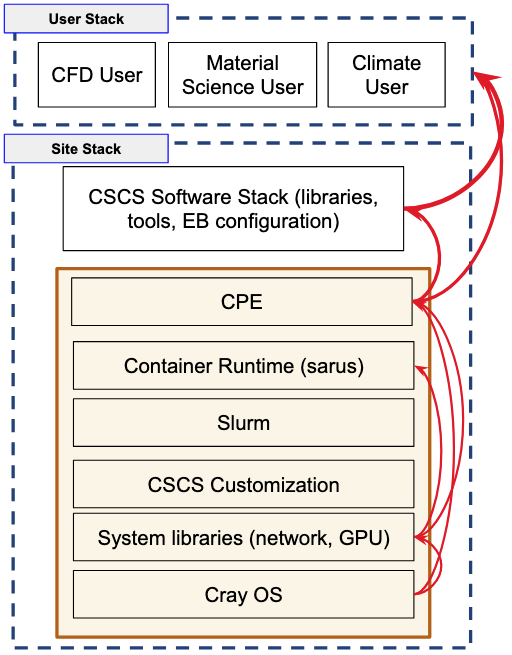
\includegraphics[width=0.4\textwidth]{./images/stack-old.png}
    \end{center}
    \caption{
        The ``standard'' HPE-EX software stack, with the Cray OS, drivers, CPE and site-specific software in the system image, site-provided software installed on a shared file system.
        User-installed software depends on the software layers underneath.
        The red arrows indicate where changes to one layer have a knock on effect on other software layers, requiring rebuilds or reconfiguration.
    }
    \label{fig:cpe-stack}
\end{figure}

To provide additional software to users, HPC centers with HPE Cray-EX systems deploy the CPE, then build additional software using the components it provides -- primarily the compiler wrappers, cray-mpich, CUDA/ROCM and widely-used libraries like FFTw and netcdf.
Centers have developed workflows that use on HPC package management tools like Spack and EasyBuild to build the software, store the configuration in git repositories, and deploy using pipelines with varying levels of automation~\cite{setonix2023,eb2016}.
This additional software is deployed to a shared file system, where it is available for users to use alongside the CPE, as illustrated in~\fig{cpe-stack}.

The downside of this approach is that installing a new version of the CPE, which is released every 6 months, is very disruptive:
\begin{itemize}
    \item changes in the CPE often require reconfiguring and rebuilding centre-provided software - the task of updating Spack and EasyBuild to use new locations and versions of CPE software is particularly time consuming;
    \item users who have built upon this foundation are similarly disrupted;
    \item installing the new CPE requires building a new OS image, typically on a test and deploymebnt (TDS) system;
    \item deployment requires rebooting the system.
\end{itemize}
These disruptions are contrary to all of our objectives for software deployment outlined in~\sect{sec:objectives}
% \item Downside: using CPE as a base layer breaks "no root", "no reboot", and "don't break user codes" tenents

This was the main motivation for CSCS persuing alternatives that don't use CPE for software deployment on Alps, that will be

We note that as of the time of writing, CPE is still available through a \lst{cray} module on the Daint cluster on Alps, for users who require it, or are still in the process of transitioning to uenv and containers.
The \lst{cray} module is the only module available to users on Alps when they first log in, and loading it loads the \lst{PrgEnv-cray} meta-module and populates the full set of available modules.

The module has caused confusion for users, because it is the only obvious software installed on the system when the first log in (unless they have read the documentation).
In \sect{sec:cpe-container} we describe how CSCS will continue providing CPE in a container, in order to improve how CPE is deployed, and help users make a more informed decision about their software environment.
